\documentclass{beamer}
\usepackage{amsmath,amsbsy,amsopn,amstext,amsfonts,amssymb}
\usepackage{isomath}
\usepackage{ulem}
%\linespread{1.6}  % double spaces lines
\usepackage{graphicx}
\usepackage{subfigure}
\usepackage{color}
\usepackage{optidef}  % define optimization problems
\usepackage{multicol}  % multiple columns
\usepackage{listings} % for python code
\usepackage{mathrsfs}

\usepackage{polynom}
\newcommand{\adj}{\mathrm{adj}}
\newcommand{\constrainedmin}[3]{
		\begin{mini*}|s|
		{#2}{#1}{}{}
		\addConstraint{#3}
		\end{mini*}
}

\newcommand{\rwbcomment}[1]{{\color{blue}RWB:#1}}
\newcommand{\defeq}{\stackrel{\triangle}{=}}
\newcommand{\abs}[1]{\left|#1\right|}
\newcommand{\norm}[1]{\left\|#1\right\|}
\newcommand{\iprod}[1]{\left<#1\right>}
\newcommand{\ellbf}{\boldsymbol{\ell}}
\newcommand{\nubf}{\boldsymbol{\nu}}
\newcommand{\mubf}{\boldsymbol{\mu}}
\newcommand{\abf}{\mathbf{a}}
\newcommand{\bbf}{\mathbf{b}}
\newcommand{\cbf}{\mathbf{c}}
\newcommand{\dbf}{\mathbf{d}}
\newcommand{\ebf}{\mathbf{e}}
\newcommand{\fbf}{\mathbf{f}}
\newcommand{\gbf}{\mathbf{g}}
\newcommand{\hbf}{\mathbf{h}}
\newcommand{\ibf}{\mathbf{i}}
\newcommand{\jbf}{\mathbf{j}}
\newcommand{\kbf}{\mathbf{k}}
\newcommand{\lbf}{\mathbf{l}}
\newcommand{\mbf}{\mathbf{m}}
\newcommand{\nbf}{\mathbf{n}}
\newcommand{\obf}{\mathbf{o}}
\newcommand{\pbf}{\mathbf{p}}
\newcommand{\qbf}{\mathbf{q}}
\newcommand{\rbf}{\mathbf{r}}
\newcommand{\sbf}{\mathbf{s}}
\newcommand{\tbf}{\mathbf{t}}
\newcommand{\ubf}{\mathbf{u}}
\newcommand{\vbf}{\mathbf{v}}
\newcommand{\wbf}{\mathbf{w}}
\newcommand{\xbf}{\mathbf{x}}
\newcommand{\ybf}{\mathbf{y}}
\newcommand{\zbf}{\mathbf{z}}
\newcommand{\Jbf}{\mathbf{J}}
\newcommand{\Acal}{\mathcal{A}}
\newcommand{\Bcal}{\mathcal{B}}
\newcommand{\Lcal}{\mathcal{L}}
\newcommand{\Ncal}{\mathcal{N}}
\newcommand{\Rcal}{\mathcal{R}}
\definecolor{darkolivegreen}{rgb}{0.33, 0.42, 0.18}

\makeatletter
\newenvironment<>{proofstart}[1][\proofname]{%
    \par
    \def\insertproofname{#1\@addpunct{.}}%
    \usebeamertemplate{proof begin}#2}
  {\usebeamertemplate{proof end}}
\newenvironment<>{proofcont}{%
  \setbeamertemplate{proof begin}{\begin{block}{}}
    \par
    \usebeamertemplate{proof begin}}
  {\usebeamertemplate{proof end}}
\newenvironment<>{proofend}{%
    \par
    \pushQED{\qed}
    \setbeamertemplate{proof begin}{\begin{block}{}}
    \usebeamertemplate{proof begin}}
  {\popQED\usebeamertemplate{proof end}}
\makeatother

\title{ECEn 671: Mathematics of Signals and Systems \\ 
Moon: Chapter 18.}
\author{Randal W. Beard}
\institute{Brigham Young University}
\date{\today}

\begin{document}

%-------------------------------
\begin{frame}
	\titlepage
\end{frame}

%-------------------------------
\begin{frame}[t]
\frametitle{Table of Contents}
\tableofcontents
\end{frame}

%%%%%%%%%%%%%%%%%%%%%%%%%%%%%%%%%%%%%%%%%%%%%%%%%%%%%%%%%%%%%%%%%
\section{Constrained Optimization}
\frame{\sectionpage}


%----------------------------------
\begin{frame}\frametitle{Constrained Optimization}
	In Chapter 14 we studied unconstrained minimization of continuously differentiable functions.
	
	\vfill
	
	In Chapter 18 we focus on constrained optimization problems.
	
	\vfill
	
	For example, given the level curves,
	\begin{center}
		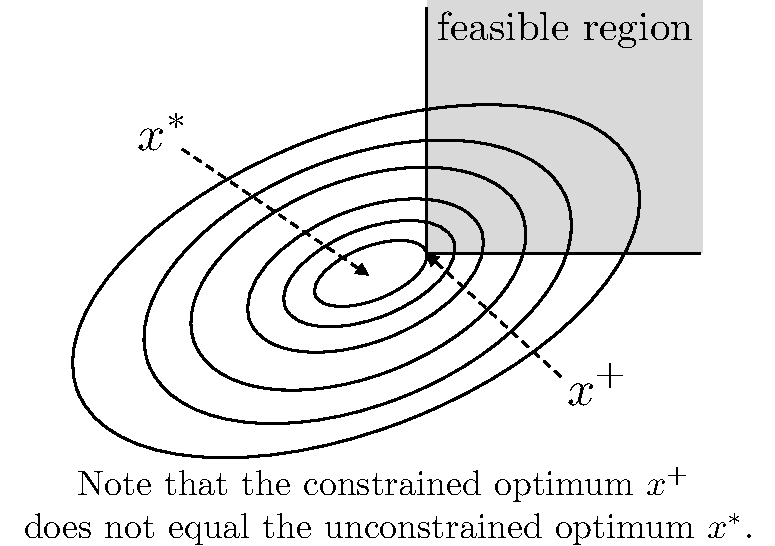
\includegraphics[width=0.5\textwidth]
			{figures/chap18_constrained_optimum}
	\end{center}
	The unconstrained optimum is $x^{\ast}$; the constained optimum is $x^{+}$.
\end{frame}

%----------------------------------
\begin{frame}\frametitle{Constrained Optimization}
	\begin{definition}
		Let $\Omega \subseteq \mathbb{R}^n$ be the feasible region.  
		Then $x^{\ast}\in \Omega$ is a \underline{local minimum} of $f:\mathbb{R}^n\to\mathbb{R}$ over $\Omega$ if $\exists \epsilon > 0$ such that 
		\[
			x \in \Omega \cap \{y\in \mathbb{R}^n:|u-x^{\ast}|<\epsilon\} \quad \implies \quad f(x) \geq f(x^{\ast}).
		\]
		If $f(x) > f(x^{\ast})$ then $x^{\ast}$ is a \underline{strict local minimum}.  
		If true for all $\epsilon > 0$ then $x^{\ast}$ is a global minimum.
	\end{definition}
	
	\vfill

	\begin{center}
		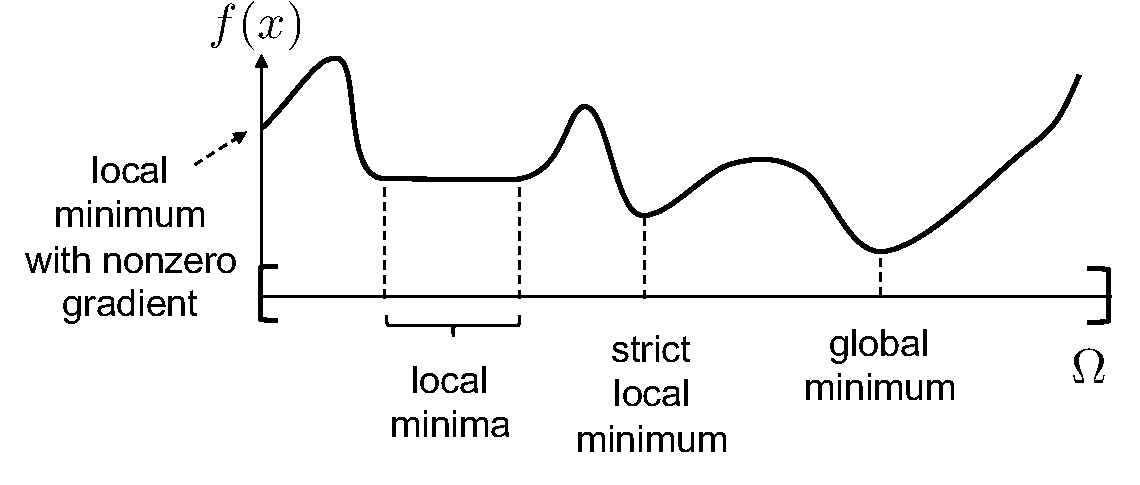
\includegraphics[width=0.6\textwidth]
			{figures/chap18_types_of_minima}
	\end{center}
\end{frame}

%----------------------------------
\begin{frame}\frametitle{Constrained Optimization}
	\begin{definition}
		Let $x \in \Omega$ and $d \in \mathbb{R}^n$, then 
		\[
			y = x+ \alpha d
		\]
		is a \underline{feasible point} if $y \in \Omega$.
	\end{definition}
	
	\vspace{0.5cm}
	
	\begin{definition}
		The vector $d$ is a \underline{feasible direction} at $x$, if $\exists\epsilon_0 > 0$ such that 
		\[
			x + \epsilon d \in \Omega
		\]		
		for every $0 \leq \epsilon \leq \epsilon_0$.
	\end{definition}
\end{frame}

%----------------------------------
\begin{frame}\frametitle{Constrained Optimization}
	Recall, if $f: \mathbb{R}^n\to\mathbb{R}$ then the gradient vector is
	\[
		\frac{\partial f}{\partial x} 
			= \nabla_x f 
			= \begin{pmatrix}
	    		\frac{\partial f}{\partial x_1}\\
	    		\vdots\\
	    		\frac{\partial f}{\partial x_n}
	  		  \end{pmatrix}
	\]
	and the Hessian matrix is
	\[ 
		\frac{\partial^2 f}{\partial x^2} 
			= \nabla^2f 
			= \begin{pmatrix}
	    		\frac{\partial^2 f}{\partial x_1^2} & \frac{\partial^2 f}{\partial x_1 \partial x_2} & \cdots & \frac{\partial^2 f}{\partial x_1 \partial x_n}\\
	    		\vdots & & & \vdots\\
	    		\frac{\partial^2 f}{\partial x_n \partial x_1} & \cdots & \cdots & \frac{\partial^2 f}{\partial x_n^2}
	  		  \end{pmatrix}.
	\]	
	If $\Omega = \mathbb{R}^n$ then a necessary condition for $x^{\ast}$ to be a local minima is that $\nabla_xf(x^{\ast})=0$.  What about constrained optimization problems?
\end{frame}

%----------------------------------
\begin{frame}\frametitle{Constrained Optimization}
	\begin{theorem}[Moon Theorem 18.1]
		Let $\Omega \subseteq \mathbb{R}^n$ and let $f:\mathbb{R}^n\to\mathbb{R}$ be $\mathcal{C}^1$ (continuously differentiable) on $\Omega$.
		
		\begin{enumerate}
		\item If $x^{\ast}$ is a local minimum of $f$ over $\Omega$, then for \underline{any} feasible direction $d \in \mathbb{R}^n$ at $x^{\ast}$
			\[ 
				\left[ \nabla_xf(x^{\ast}) \right]^\top d \geq 0 
			\]
		\item If $x^{\ast}$ is an interior point of $\Omega$, then 
			\[ 
				\nabla f(x^{\ast}) = 0.
			\]
		\item If in addition, $f \in \mathcal{C}^2$ and $\nabla_x f(x^{\ast})^\top d = 0$, then 
			\[ 
				d^\top \nabla^2f(x^{\ast})d \geq 0 
			\]
			Note that this is a weaker condition than psd Hessian.
		\end{enumerate}		
	\end{theorem}
\end{frame}

%----------------------------------
\begin{frame}\frametitle{Proof of Theorem 18.1}
	1. By Taylor series expansion,
	\begin{align*}
		& f(x^{\ast} + \epsilon d) = f(x^{\ast}) + \epsilon\nabla_xf(x^{\ast})^\top d+ O(\epsilon) \\
		\implies & f(x^{\ast}+\epsilon d) - f(x^{\ast}) = \epsilon\nabla_xf(x^{\ast})^\top d + O(\epsilon) 
	\end{align*}
	Since $x^{\ast}$ is a local minimum, for $\epsilon$ sufficiently small we must have that
	\begin{align*}
		\implies & f(x^{\ast} + \epsilon d) - f(x^{\ast}) \geq 0 \\
		\implies & \nabla_xf(x^{\ast})^\top d \geq 0.
	\end{align*}	
\end{frame}

%----------------------------------
\begin{frame}\frametitle{Proof of Theorem 18.1, cont.}
	2.  If $x^{\ast}$ is an interior point then every $d \in \mathbb{R}^n$ is feasible at $x^{\ast}$, i.e.
	\[ 
		\iprod{\nabla_xf(x^{\ast}), d }_{\mathbb{R}^n} = 0, \qquad \forall d\in\mathbb{R}^n. 
	\]
	Therefore,
	\begin{align*}
	  & \nabla_xf(x^{\ast})^\top d \geq 0 
	  	\quad \text{and} \quad 
	  	\nabla_xf(x^{\ast})^\top (-d) \geq 0\\
	  \implies & \nabla_xf(x^{\ast})^\top d = 0, \quad \forall d\in\mathbb{R}^n \\
	  \implies &  \nabla_xf(x^{\ast}) = 0
	\end{align*}
	since $R^n$ is a finite dimensional vector space	.
\end{frame}

%----------------------------------
\begin{frame}\frametitle{Proof of Theorem 18.1, cont.}
	3.  If $\nabla_xf(x^{\ast})^\top d = 0$ then the Taylor series for $f$ is
	\begin{align*}
		& f(x^{\ast}+\epsilon d) = f(x^{\ast}) + \epsilon^2d^\top \nabla^2f(x^{\ast})d + O(\epsilon^2) \\
		\implies &  0 \leq f(x^{\ast} + \epsilon d) - f(x^{\ast}) = \epsilon^2d^\top \nabla^2f(x^{\ast})d + O(\epsilon^2) \\
		\implies & d^\top \nabla^2f(x^{\ast})d \geq 0.
	\end{align*}
	\begin{center}
		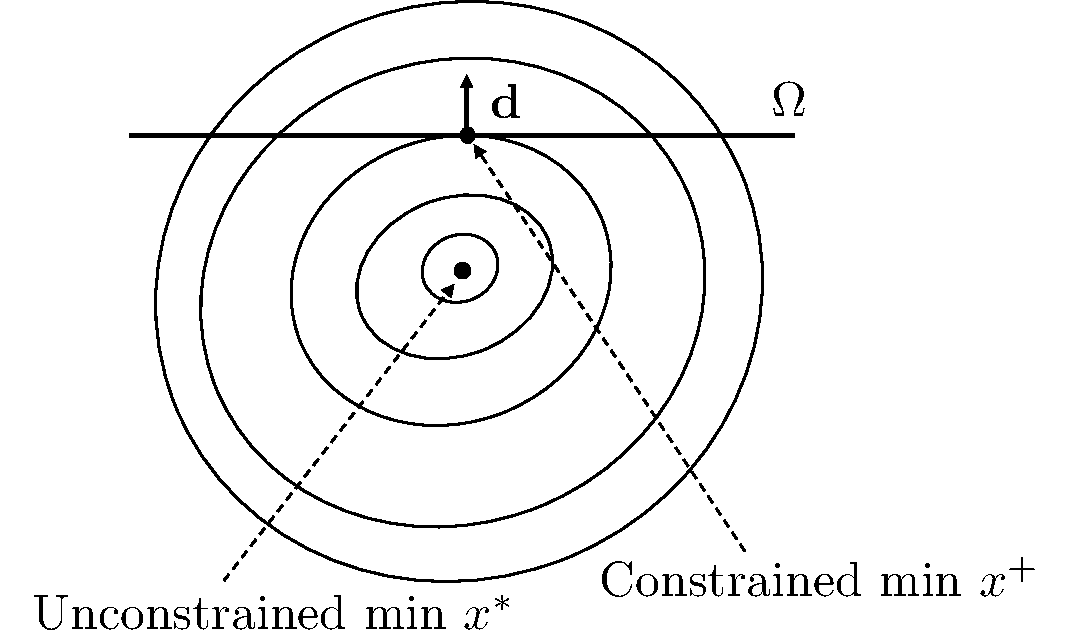
\includegraphics[width=0.5\textwidth]
			{figures/chap18_linear_constraint}
	\end{center}

	Note:  Any feasible $d$ points uphill.
	
	Note:  The function is concave in feasible region.
\end{frame}

%----------------------------------
\begin{frame}\frametitle{Constrained Optimization: Sufficient Conditions}
	\underline{Are there sufficient conditions?}
	
	\vfill
	
	First, suppose that the constraints are not active, i.e. $x^{\ast}$ is an interior point of $\Omega$.  (We will consider the active constraint case later.)
	
	\vfill
	
	\begin{theorem}[Moon Theorem 18.2]
		Let $f \in \mathcal{C}^2$ on $\Omega$ and let $x^{\ast}$ be an interior point of $\Omega$.  If $\nabla f(x^{\ast}) = 0$ and $\nabla^2f(x^{\ast})$ is positive definite then $x^{\ast}$ is a strict local minimum of $f$.
	\end{theorem}
\end{frame}

%----------------------------------
\begin{frame}\frametitle{Constrained Optimization: Sufficient Conditions: Proof}
	\begin{proof}
		Let $d$ be any unit vector in $\mathbb{R}^n$ then 
		\begin{align*}
			& 	f(x^{\ast} + \epsilon d) = f(x^{\ast}) + \epsilon\nabla f(x^{\ast})^\top d + \epsilon^2d^\top \nabla^2f(x^{\ast})d + O(\epsilon^2) \\
			\implies & 
			f(x^{\ast} + \epsilon d)  - f(x^{\ast}) = \epsilon^2d^\top \nabla^2f(x^{\ast})d + O(\epsilon^2)
		\end{align*}
	
		Since $\nabla^2f(x^{\ast})$ is positive definite, it follows that for $\epsilon$ sufficiently small
		\[ 
			f(x^{\ast}+\epsilon d) - f(x^{\ast}) > 0,
		\]
		which implies that $x^{\ast}$ is a strict local minimum. 	
	\end{proof}
	
	\vfill
	
	{\bf Note:} we cannot generalize this theorem to the case when $\nabla^2f(x^{\ast})$ is p.s.d..  Why?
\end{frame}

%%%%%%%%%%%%%%%%%%%%%%%%%%%%%%%%%%%%%%%%%%%%%%%%%%%%%%%%%%%%%%%%%
\section{General Constrained Optimization}
\frame{\sectionpage}

%----------------------------------
\begin{frame}\frametitle{Constrained Optimization}
	In general we have two types of constraints:
	\begin{enumerate}
		\item 	
			Equality constraints of the form
			\[ 
				h_i(x) = 0 
			\]
			For example:
			\[
				h_1(x) \defeq x_1^2 + x_1x_2x_3 + \tan(x_3)\cos(x_2) = 0
			\]
			
		\item 
			Inequality constraints of the form
			\[ 
				g_i(x) \leq 0 
			\]
			For example
			\begin{align*}
				& x_1 \geq 0, & x_2 \geq 0 \\
				\implies & g_1(x)\defeq -x_1 \leq 0, & g_2(x) \defeq -x_2 \leq 0 
			\end{align*}
			\end{enumerate}
\end{frame}

%----------------------------------
\begin{frame}\frametitle{Constrained Optimization}
	In fact a region $\Omega \subset \mathbb{R}^n$ can always be described by inequality constraints.

	\vfill
		
	\begin{example}
		\begin{columns}
			\begin{column}{0.35\textwidth}
				Feasible Region $\Omega$:
				\begin{align*}
					(x-\ybf_1)^\top \nbf_1 &\leq 0	\\
					(x-\ybf_2)^\top \nbf_2 &\leq 0	\\
					(x-\ybf_3)^\top \nbf_3 &\leq 0
				\end{align*}
			\end{column}
			\begin{column}{0.65\textwidth}
				\begin{center}
					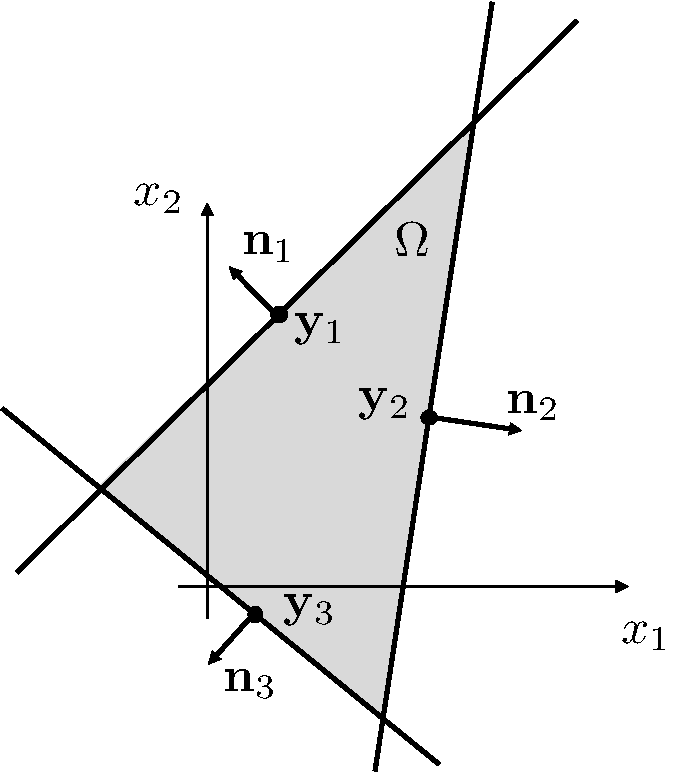
\includegraphics[width=0.5\textwidth]
						{figures/chap18_inequality_constraints}
				\end{center}
			\end{column}
		\end{columns}
		Where $\nbf_i$ is a vector normal to the linear constraint.	
	\end{example}
\end{frame}

%----------------------------------
\begin{frame}\frametitle{Constrained Optimization}
	A general constrained optimization problem can be written as
	\begin{mini*}|s|
		{x\in\Omega}{f(x)}{}{}
		\addConstraint{h_1(x)=0}
		\addConstraint{\vdots}
		\addConstraint{h_m(x)=0}
		\addConstraint{g_1(x)\leq 0}		
		\addConstraint{\vdots}
		\addConstraint{g_p(x)\leq 0}
	\end{mini*}
\end{frame}

%----------------------------------
\begin{frame}\frametitle{Constrained Optimization}
	Letting 
		\begin{align*}
			\hbf &= (h_1 \ldots h_m)^\top \\
			\gbf &= (g_1 \ldots g_p)^\top,		
		\end{align*}
 	we have
	\begin{mini*}|s|
		{x\in\Omega}{f(x)}{}{}
		\addConstraint{\hbf(x)=0}
		\addConstraint{\gbf(x)\leq 0}		
	\end{mini*} 	
	
	Equality constraints are easier to deal with than inequality constraints.
	
	\vfill
	
	We will first treat equality constraints, then inequality constraints.
	
\end{frame}

%%%%%%%%%%%%%%%%%%%%%%%%%%%%%%%%%%%%%%%%%%%%%%%%%%%%%%%%%%%%%%%%%
\section{Equality Constraints: Lagrange Multipliers}
\frame{\sectionpage}

%----------------------------------
\begin{frame}\frametitle{Equality Constraints: Lagrange Multipliers}
	Several geometric insights help:
	
	{\color{blue}Insight  \#1} 
	\begin{itemize}
		\item Geometrically what do the constraints $\hbf(x) = 0$ look like?
		\item What if $\hbf$ is linear, i.e. $\hbf(x) = Hx = 0$ where $H:\mathbb{R}^n\to\mathbb{R}^m$.
		\item The constraint implies that $x$ must be in the null space of $H$, which is a linear space of dimension $n-m$, i.e. an $n-m$ dimensional hyperplane.
		\item In general, $\hbf(x)=0$ is an $n-m$ dimensional hypersurface in $\mathbb{R}^n$.
	\end{itemize}

	\begin{center}
		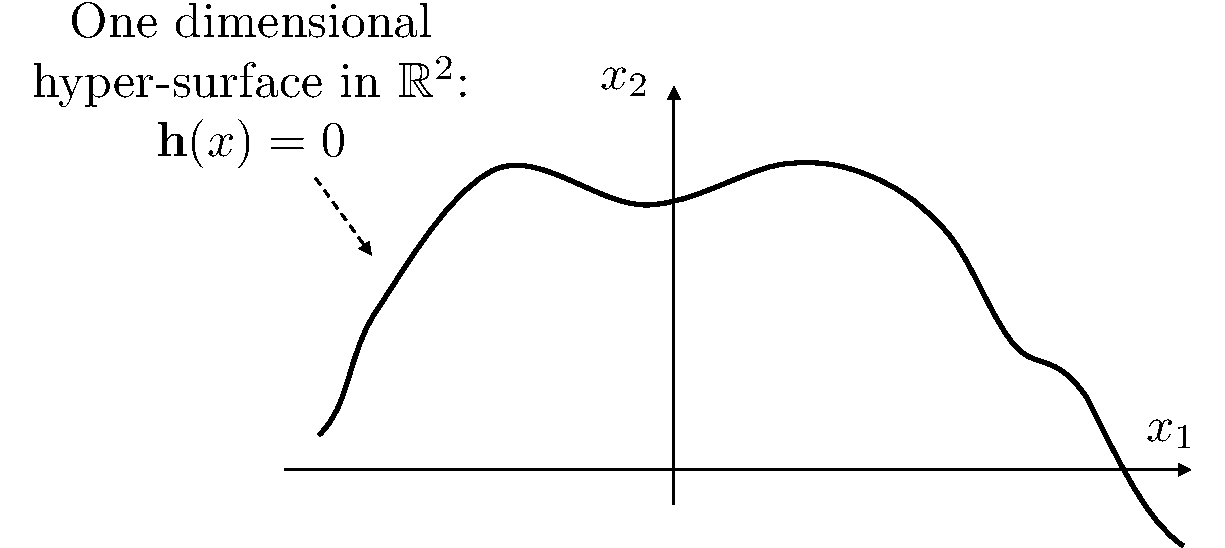
\includegraphics[width=0.5\textwidth]
			{figures/chap18_hypersurface}
	\end{center}
	
\end{frame}

%----------------------------------
\begin{frame}\frametitle{Equality Constraints: Lagrange Multipliers}
	{\color{blue}Insight  \#2}
	\begin{center}
		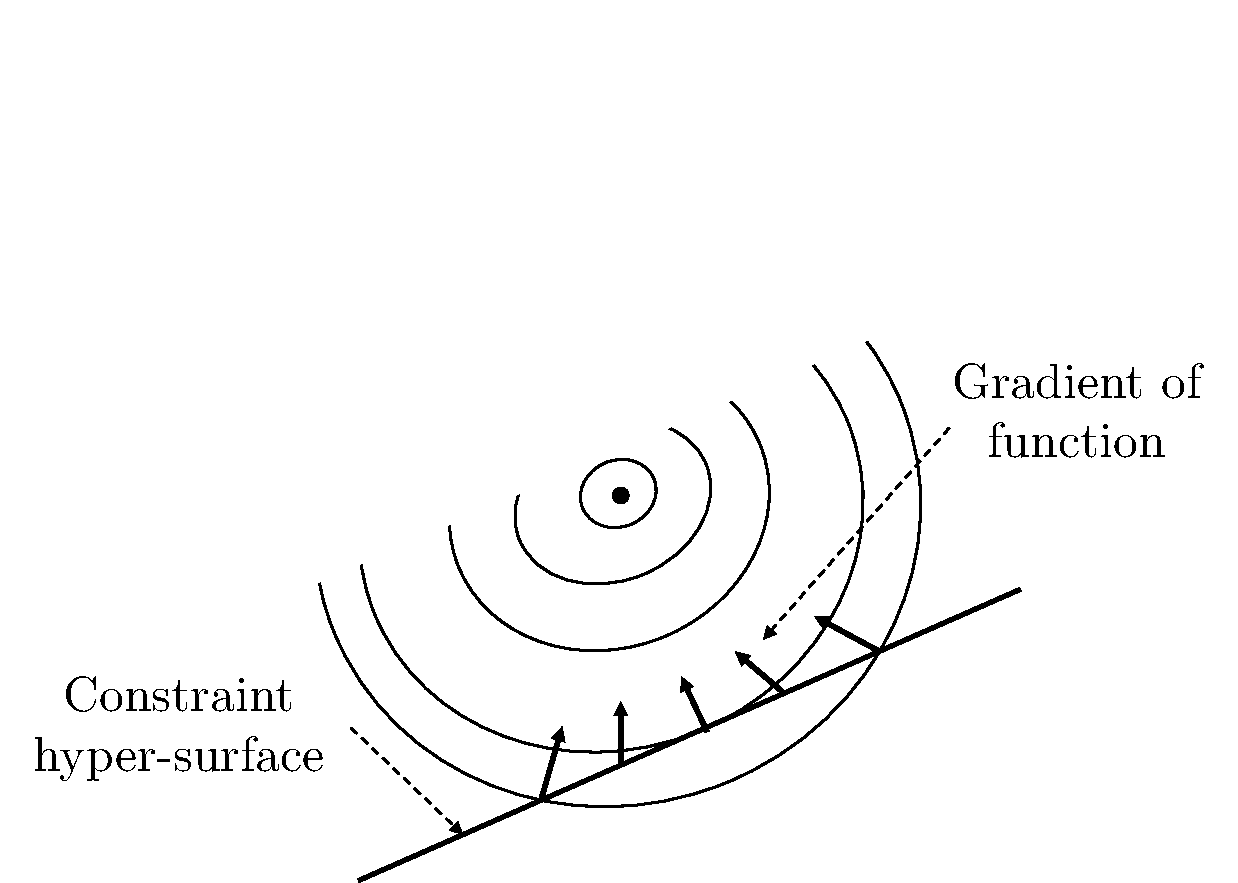
\includegraphics[width=0.5\textwidth]
			{figures/chap18_gradient_on_constraint}
	\end{center}
	
	At a constrained minimum the gradient is orthogonal to the hypersurface.
\end{frame}

%----------------------------------
\begin{frame}\frametitle{Equality Constraints: Lagrange Multipliers}
	To formalize, we need some definitions.
	
	Let $\mathbb{S}$ be a hyper-surface of dimension $n-m$.  Let $x$ be a curve on $\mathbb{S}$ continuously parameterized by $\xi \in [a,b]$, i.e. $x(\xi) \in \mathbb{S}$.
	
	\begin{center}
		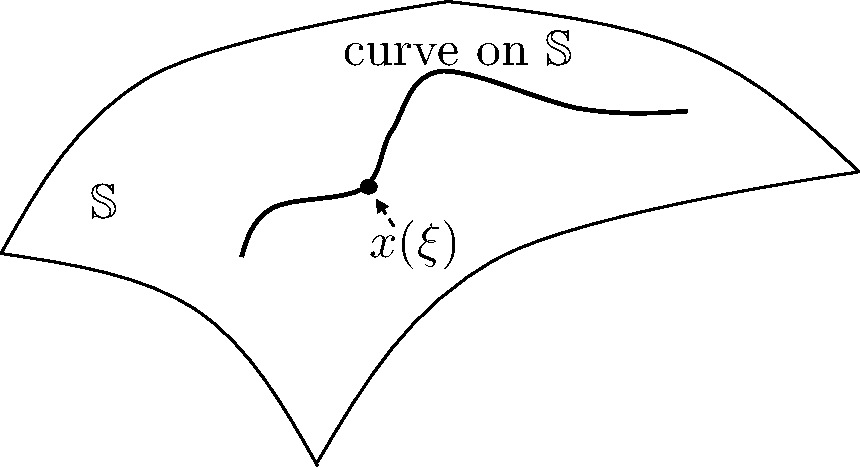
\includegraphics[width=0.5\textwidth]
			{figures/chap18_curve_on_S}
	\end{center}
	
	The derivative of the curve at $x(\xi_0)$ is 
	\[
		\dot{x}(\xi_0) = \frac{d}{d\xi}x(\xi_0).
	\]	
\end{frame}

%----------------------------------
\begin{frame}\frametitle{Equality Constraints: Lagrange Multipliers}
	\begin{definition}
		The \underline{tangent plane} to a surface $\mathbb{S}$ at $x \in \mathbb{S}$ is the span of the derivatives of all the differentiable curves on $\mathbb{S}$ at $x$.
	\end{definition}
	
	\vfill

	The problem with this definition is that it is not constructive, i.e. it doesn't give us a good way to actually construct the tangent plane.
	
\end{frame}

%----------------------------------
\begin{frame}\frametitle{Equality Constraints: Lagrange Multipliers}
	To construct the tangent plane, recall that the gradient of $\hbf(x)$ is orthogonal to level curves of $\hbf(x)$:
	\begin{center}
		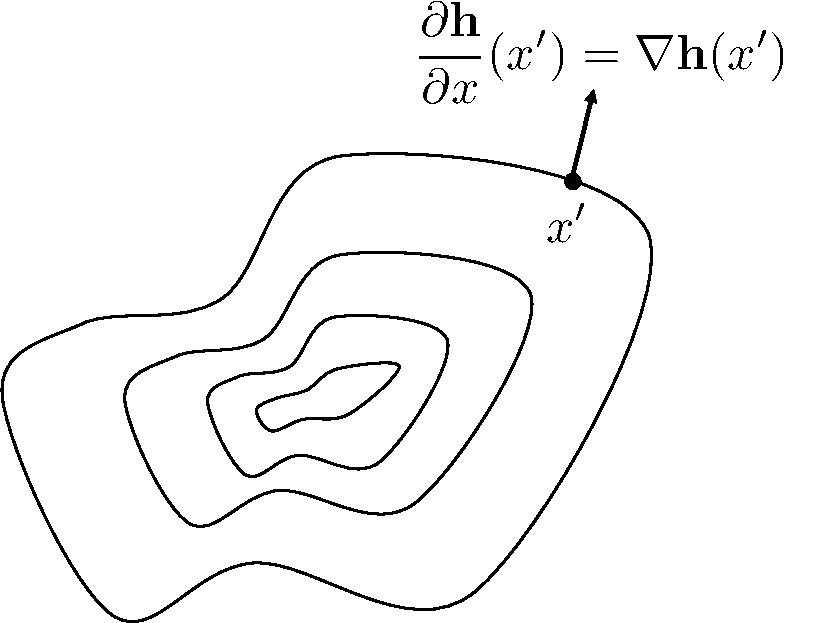
\includegraphics[width=0.3\textwidth]
			{figures/chap18_gradient_h}
	\end{center}	
	Also recall that the formula for the plane is
	\[
		\left\{ y\in \mathbb{R}^n \mid \nbf^\top (y-x^{\ast})=0 \right\}.
	\]
	\begin{center}
		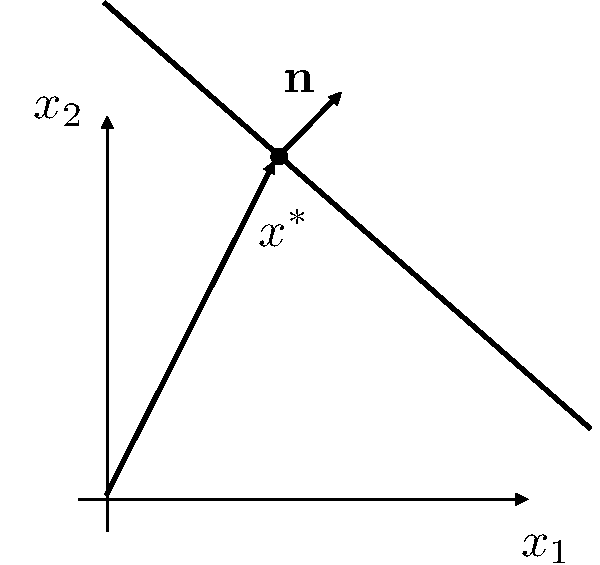
\includegraphics[width=0.3\textwidth]
			{figures/chap18_line}
	\end{center}
\end{frame}

%----------------------------------
\begin{frame}\frametitle{Equality Constraints: Lagrange Multipliers}
	Therefore the tangent plane of $h(x)$ at $x^{\ast}$ is given by
	\[ 
		P = \{ y\in \mathbb{R}^n \mid \nabla \hbf^\top (x^{\ast})(y-x^{\ast}) =0 \} 
	\]
	where $\nabla \hbf^\top (x^{\ast})$ defines an $n-m$ dimensional plane if the rows are linearly independent.

	\begin{definition}
		When the gradient vectors $\nabla h_1, \nabla h_2, \ldots, \nabla h_m$ are linearly independent at $x^{\ast}$, $x^{\ast}$ is called a \underline{regular point}.	 
	\end{definition}

	\vfill
	
	We will always assume ``regularity'' of the constraints.
\end{frame}
	
%----------------------------------
\begin{frame}\frametitle{Equality Constraints: Lagrange Multipliers}
	\begin{lemma}[Moon Lemma 18.1]
		Let $x(\xi)$ be a curve on $\hbf(x) = 0$ such that 
		\[
			\left. x(\xi)\right|_{\xi=0} = x^{\ast},
		\] 
		is a constrained local minimum of $f$.		
		Then 
		\[
			\left. \displaystyle\frac{d}{d\xi}f(x(\xi))\right|_{\xi=0} = 0.
		\]		
	\end{lemma}
	Geometry: at point $p$, $f$ is neither increasing nor decreasing along $x(\xi)$.
	\begin{center}
		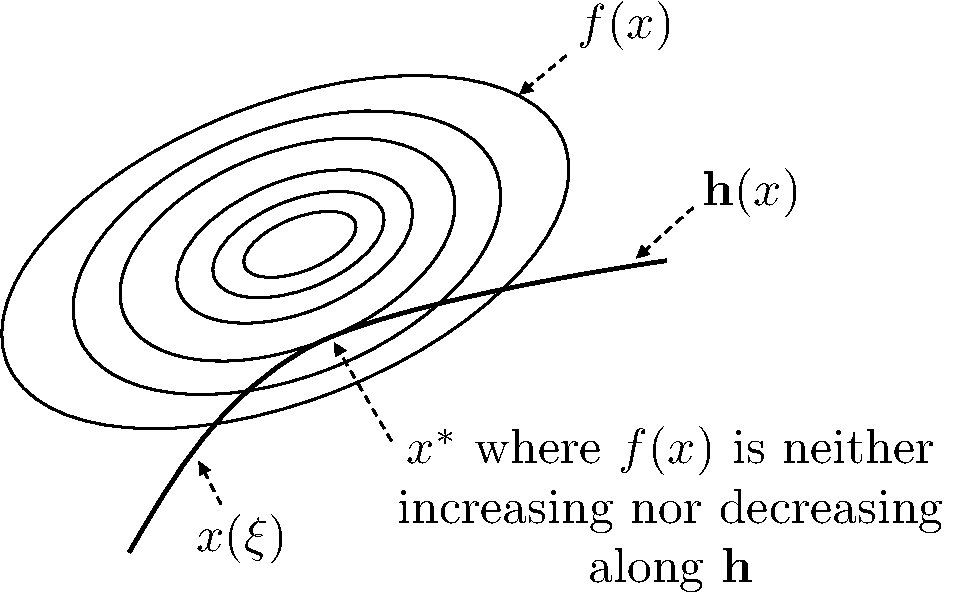
\includegraphics[width=0.4\textwidth]
			{figures/chap18_constraint_along_h}
	\end{center}
		
\end{frame}

%----------------------------------
\begin{frame}\frametitle{Equality Constraints: Lagrange Multipliers: Proof}
	\begin{proof}
		Expanding $f(x(\xi))$ in a Taylor series:
		\[ 
			f(x(\xi)) = \left. f(x(0)) + \xi\frac{d}{d\xi}f(x(\xi))\right|_{\xi=0} + O(|\xi|) 
		\]
		If $f(x(0))$ is a local minimum then for $\abs{\xi}$-small
		\[ 
			\left. \xi\frac{d}{d\xi}f(x(\xi))\right|_{\xi =0} \geq 0 
		\]
		for all $\xi$ both positive and negative.  Therefore
		\[ 
			\left. \frac{d}{df}f(x(\xi))\right|_{\xi=0} = 0 
		\]
		where
		\( 
			\frac{d}{d\xi}f(x(\xi)) = \nabla^\top f(x(\xi)) \dot{x}(\xi)
		\)
		and $\dot{x}(\xi)$ is an element of the tangent plane.
	\end{proof}
\end{frame}

%----------------------------------
\begin{frame}\frametitle{Equality Constraints: Lagrange Multipliers}
	\begin{lemma}[Moon Lemma 18.2]
		If $x^{\ast}$ is a regular point of $\hbf(x) = 0$ \underline{and} a local constrained minimum, then 
		\[ 
			\nabla \hbf^\top (x^{\ast})y = 0 \Rightarrow \nabla f^\top (x^{\ast})y = 0 
		\]
		i.e. if $y$ is in the tangent plane of $\hbf$ at $x^{\ast}$, then $y$ is orthogonal to the gradient of $f$.	
	\end{lemma}
	\begin{center}
		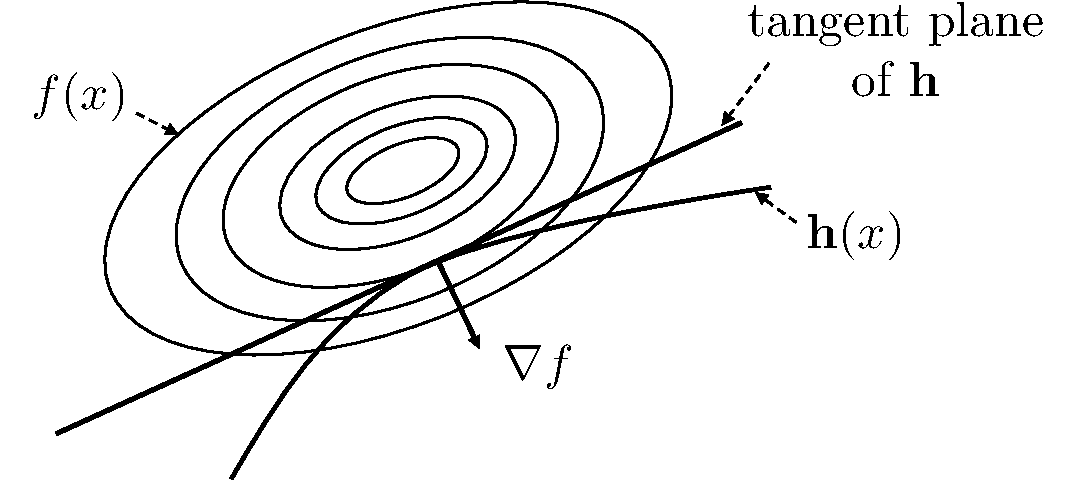
\includegraphics[width=0.5\textwidth]
			{figures/chap18_tangent_plane_of_h}
	\end{center}	
\end{frame}

%----------------------------------
\begin{frame}\frametitle{Proof of Lemma 18.2}
	\begin{proof}
		Translate the coordinate system such that $x^{\ast} = 0$.  Regularity implies that the tangent plane is given by 
		\[ 
			P(x^{\ast}) \defeq \{ z\in \mathbb{R}^n \mid \nabla \hbf^\top (x^{\ast})z = 0 \} 
		\]
		Let $y \in P(x^{\ast})$ then 
		\[
			\nabla \hbf^\top (x^{\ast}) y = 0.
		\]
		
		\vfill
		
		Now choose a smooth curve $x(\xi)$ on $\hbf(x) = 0$ such that $x(0) = x^{\ast}$ and $\dot{x}(0) = y$.
		
		\vfill
		
		From Lemma 18.1, $\nabla f^\top (x^{\ast})y = 0$. 
	\end{proof}
\end{frame}

%----------------------------------
\begin{frame}\frametitle{Key Insight}
	At a constrained local minimum $\nabla f(x^{\ast})$ and the columns of $\nabla \hbf(x^{\ast})$ are parallel, i.e., there is some scalar $\mu_i$ such that
	\begin{align*}
		& \nabla f(x^{\ast}) = \mu_i\nabla h_i(x^{\ast}) \qquad i= 1,\ldots,m \\
		\implies & m\nabla f(x^{\ast}) = \sum_{i=1}^m \mu_i \nabla h_i (x^{\ast}) \\
		\implies & \nabla f(x^{\ast}) - \sum_{i=1}^m \frac{\mu_i}{m}\nabla h_i(x^{\ast}) = 0\\
		\implies & \fbox{$\nabla f(x^{\ast}) + \nabla \hbf(x^{\ast}) \lambda = 0$}
	\end{align*}
	where 
	\[
		\lambda = \begin{pmatrix}
	    			-\frac{\mu_1}{m} &
	    			\dots &
	    			-\frac{\mu_m}{m}
	  			  \end{pmatrix}^\top.
	\]
	The vector $\lambda \in \mathbb{R}^m$ is called the \underline{Lagrange Multiplier}.	
\end{frame}

%----------------------------------
\begin{frame}\frametitle{Necessary Conditions}
	\begin{theorem}[Moon Theorem 18.3 (Necessary conditions for equality constraints)]
		Let $x^{\ast}$ be a local extremum of $f$ subject to the constraints $h(x) = 0$, and let $x^{\ast}$ be a regular point.  Then there is a $\lambda \in \mathbb{R}^n$ such that
		\[ 
			\nabla f(x^{\ast}) + \nabla \hbf(x^{\ast})\lambda = 0.
		\]
	\end{theorem}	
	\begin{corollary}
		Let 
		\[ 
			L(x,\lambda) = f(x) + \hbf^\top(x)\lambda.
		\]
		Then if $x^{\ast}$ is a regular local extremum, then
		\[ 
			\nabla_x L(x^{\ast},\lambda^{\ast}) = \frac{\partial L}{\partial x}(x^{\ast},\lambda^{\ast}) = 0 
		\]
		and
		\[ 
			\nabla_{\lambda}L(x^{\ast},\lambda^{\ast}) = \frac{\partial L}{\partial \lambda}(x^{\ast},\lambda^{\ast}) = 0.
		\]
	\end{corollary}
\end{frame}
	
%----------------------------------
\begin{frame}\frametitle{Proof of Theorem 18.3}
	\begin{proof}
		\begin{eqnarray}
		\label{eqn18.3.1} \frac{\partial L}{\partial x} = \nabla f(x^{\ast}) + \nabla h(x^{\ast}) \lambda^{\ast} = 0 \\
		\label{eqn18.3.2} \frac{\partial L}{\partial \lambda} = h(x^{\ast}) = 0
		\end{eqnarray}
		Equation (\ref{eqn18.3.2}) implies that the constraints are satisfied.
		
		Equation (\ref{eqn18.3.1}) comes from Theorem 18.3.
	\end{proof}
\end{frame}

%----------------------------------
\begin{frame}\frametitle{Lagrange Multipliers: Example 1}
	\begin{mini*}|s|
		{}{x_1^2 + x_2^2}{}{}
		\addConstraint{x_1 + x_2 = 2}
	\end{mini*}
	\begin{center}
		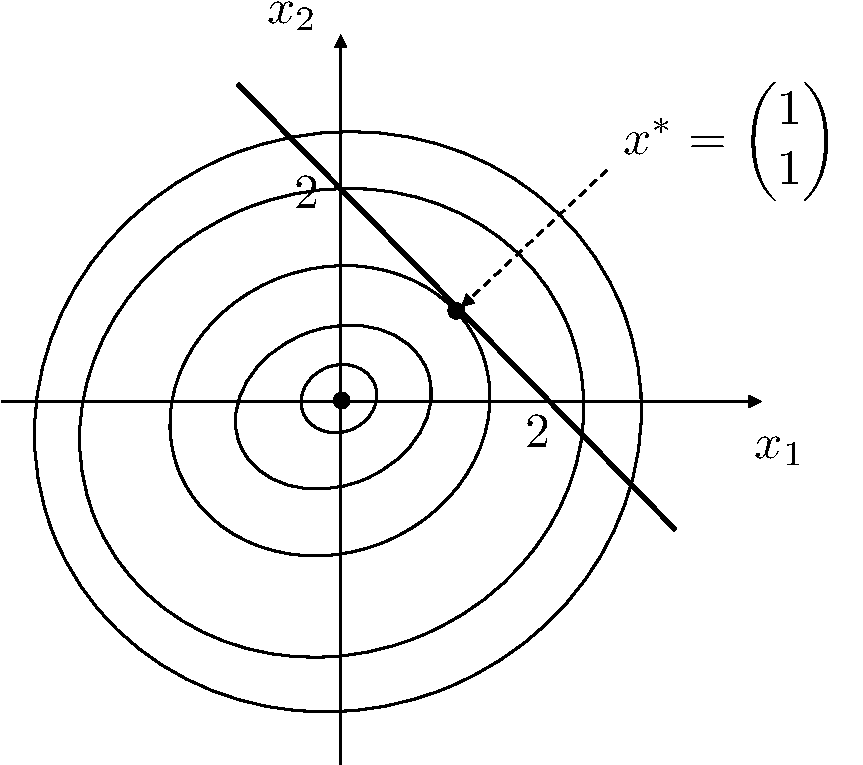
\includegraphics[width=0.5\textwidth]
			{figures/chap18_example1}
	\end{center}
	The Lagrangian is
	\[ 
		L = x_1^2 + x_2^2 + \lambda(x_1 + x_2 - 2). 
	\]	
\end{frame}
	
%----------------------------------
\begin{frame}\frametitle{Lagrange Multipliers: Example 1, cont.}
	The necessary conditions for a minimum are
	\begin{align*}
		\frac{\partial L}{\partial x_1} &= 2x_1 + \lambda = 0 \quad \implies x_1 = -\frac{\lambda}{2}\\
		\frac{\partial L}{\partial x_2} &= 2x_2 + \lambda = 0 \quad \implies x_2 = -\frac{\lambda}{2}\\
		\frac{\partial L}{\partial \lambda} &= x_1 + x_2 - 2 = 0 \quad \implies -\lambda - 2 = 0.
	\end{align*}
	Therefore $\lambda = -2$, $x_1 = 1$, $x_2 = 1$, which implies that 
	\[
			x^{\ast} 
				= 
				\begin{pmatrix}
	      			1 \\ 1
	    		\end{pmatrix}
	\]
	as expected.	
\end{frame}

%----------------------------------
\begin{frame}\frametitle{Lagrange Multipliers: Example 18.4.7 (Maximum Entropy)}
	Let $\mathbb{X}$ be a random variable with probability mass function $p(\mathbb{X}=x_i) = p_i \qquad i = 1, \ldots, m$,
	
	Then, the entropy of $\mathbb{X}$ is defined as
	\[ 
		H = -\sum_{i=1}^m p_i\log p_i 
	\]	
	Question:  Which pmf has maximum entropy?
	
	\vfill
	
	To answer, lets solve the optimization problem:
	\begin{maxi*}|s|
		{}{H}{}{}
		\addConstraint{\sum p_i = 1}
		\addConstraint{p_i \geq 0}
	\end{maxi*}
\end{frame}

%----------------------------------
\begin{frame}\frametitle{Lagrange Multipliers: Example 18.4.7 (Maximum Entropy)}
	Lets ignore the inequality constraint for now and go back later.
	
	The Lagrangian is
	\[ 
		L = -\sum p_i \log p_i + \lambda(\sum p_i - 1) 
	\]
	The necessary conditions are
	\begin{align*}
		\frac{\partial L}{\partial p_i} &= 0 \qquad i = 1, \ldots, m\\
		\frac{\partial L}{\partial \lambda} &= 0
	\end{align*}
	where
	\begin{align*}
		& \frac{\partial L}{\partial p_i} = -\log p_i - 1 + \lambda = 0 \qquad i = 1, \ldots, m\\
		\implies & \lambda = 1+\log p_i\\
		\implies & \log p_i = \lambda - 1.
	\end{align*}	
\end{frame}

%----------------------------------
\begin{frame}\frametitle{Lagrange Multipliers: Example 18.4.7 (Maximum Entropy)}
	So $p_i$ must be constant for all $i$.  The constant $\sum p_i = 1 \Rightarrow p_i = \frac{1}{n} \geq 0$, so $p_i$ satisfies the inequality constraint.
	
	\vfill
	
	In other words: the uniform pmf maximizes entropy.
	
	\vfill
	
	In other words: all possibilities are equally likely.	
\end{frame}

%----------------------------------
\begin{frame}\frametitle{Lagrange Multipliers: Example: Constrained Least Squares}
	Given an ellipsoid and a point $y$ outside the ellipsoid, find the point $z$ in the ellipsoid nearest to $y$.\\
	\begin{center}
		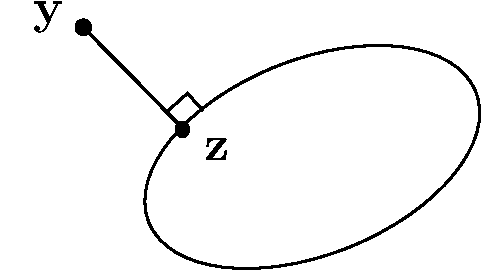
\includegraphics[width=0.5\textwidth]
			{figures/chap18_closest_point_to_set}
	\end{center}
	The equation for an ellipsoid is given by
	\[ 
		E = \{ z\in \mathbb{R}^n : z^\top L^\top Lz \leq 1.
	\]	
\end{frame}

%----------------------------------
\begin{frame}\frametitle{Lagrange Multipliers: Example: Constrained Least Squares}
	So we need to solve the following constrained optimization problem:
	\begin{mini*}|s|
		{z\in\mathbb{R}^n}{\norm{z-y }}{}{}
		\addConstraint{z^\top L^\top Lz = 1}
	\end{mini*}
	The Lagrangian is
	\[ 
		L = (y - z)^\top (y - z) + \lambda(z^\top L^\top Lz - 1) 
	\]
	
\end{frame}

%----------------------------------
\begin{frame}\frametitle{Lagrange Multipliers: Example: Constrained Least Squares}
	The necessary conditions are
	\begin{align*}
		\frac{\partial L}{\partial z} &= -2(y - z) + 2\lambda L^\top Lz = 0 \\
		\frac{\partial L}{\partial \lambda} &= z^\top L^\top Lz - 1 = 0
	\end{align*}
	The first equations gives
	\begin{align*}
		& (I + \lambda L^\top L)z = y \\
		\implies & z = (I + \lambda L^\top L)^{-1}y.
	\end{align*}
	Therefore, $\lambda$ must satisfy
	\[ 
		g(\lambda) = y^\top (I+\lambda L^\top L)^{-1}L^\top L(I + \lambda L^\top L)^{-1}y = 1 
	\]
	which must be solved numerically using a  root finding technique using e.g. Newton's method.	
\end{frame}

%----------------------------------
\begin{frame}\frametitle{Lagrange Multipliers: Example}
	Consider the following optimization problem:
	\begin{mini*}|s|
		{x\in\mathbb{R}^n}{\frac{1}{2}x^\top Ax}{}{}
		\addConstraint{Bx = c}
	\end{mini*}		
	where $A\in\mathbb{R}^{n\times n}$, 
	$B\in\mathbb{R}^{m\times n}$, 
	$c \in \mathbb{R}^{m}$.
	
	The Lagrangian is
	\[ 
		L = \frac{1}{2}x^\top Ax + \lambda^\top (Bx - c) 
	\]
\end{frame}

%----------------------------------
\begin{frame}\frametitle{Lagrange Multipliers: Example}
	The necessary conditions are
	\begin{align*}
		\frac{\partial L}{\partial x} &= Ax + B^\top \lambda = 0 \\
		\frac{\partial L}{\partial \lambda} &= Bx - c = 0
	\end{align*}
	If $A$ is invertible, then
	\begin{align*}
		& x = -A^{-1}B^\top \lambda	\\
		\implies & -BA^{-1}B^\top \lambda = c.
	\end{align*}
	If $BA^{-1}B^\top$ is invertible then
	\begin{align*}
		& 	\lambda = -(BA^{-1}B^\top )^{-1}c \\
		\implies & x = A^{-1}B^\top (BA^{-1}B^\top )^{-1}c
	\end{align*}
	which is the weighted norm pseudo-inverse.	
\end{frame}

%%%%%%%%%%%%%%%%%%%%%%%%%%%%%%%%%%%%%%%%%%%%%%%%%%%%%%%%%%%%%%%%%
\section{Sufficient Conditions}
\frame{\sectionpage}

%----------------------------------
\begin{frame}\frametitle{Lagrange Multipliers: Sufficient Conditions}
	The necessary conditions tell us where a local extremum might exist, but not whether it is a local min, max, or saddle point.
	
	\vfill
	
	Are there sufficient conditions for constrained optimization problems?	
\end{frame}

%----------------------------------
\begin{frame}\frametitle{Lagrange Multipliers: Sufficient Conditions}
	For the unconstrained problem, we look at the Hessian of $f$ for sufficient conditions.  For unconstrained problems we look at the second derivative of $L$ with respect to $x$.
	
	\vfill
	
	\[ 
		\underbrace{L}_{1\times 1} = \underbrace{f}_{1\times 1} + \underbrace{\lambda^\top }_{1\times m}\underbrace{h}_{m\times 1} = f + \sum_{i=1}^m\lambda_i h_i 
	\]
	so
	\[ 
		\underbrace{\nabla_x L}_{n\times 1} = \underbrace{\nabla_xf}_{n\times 1} + \underbrace{\nabla h}_{n\times m}\underbrace{\lambda}_{m\times 1} = \nabla_xf + \sum_{i=1}^m\lambda_i\nabla_x h_i 
	\]
	\[ 
		\nabla_{xx}^2L = \nabla_{xx}^2f + \sum_{i=1}^m\lambda_i\nabla_{xx}^2 h_i  
	\]
	We will drop the $xx$ notation (unless not obvious) to get
	
	\[ 
		\fbox{$\nabla^2L = \nabla^2f + \displaystyle\sum_{i=1}^m\lambda_i\nabla^2h_i$}
	\]	
\end{frame}

%----------------------------------
\begin{frame}\frametitle{Lagrange Multipliers: Sufficient Conditions}
	Let $P(x^{\ast}) = \{ y\in \mathbb{R}^n \mid \nabla h(x^{\ast})y = 0 \}$ be the tangent plane at $x^{\ast}$.

	\begin{theorem}[Moon Theorem 18.4]
		Let $f$ and $h$ be $C^2$
		
		1. (Necessity) Suppose that $x^{\ast}$ is a local constrained min of $f$ and that $x^{\ast}$ is regular.  Then $\exists \lambda$ such that
		\[ 
			\nabla f(x^{\ast}) + \nabla h(x^{\ast})\lambda = 0. 
		\]
		
		2. (Sufficiency)  If 
		\begin{enumerate}
		  \item $h(x^{\ast})$ = 0
		  \item $\exists \lambda$ such that $\nabla f(x^{\ast}) + \nabla h(x^{\ast}) \lambda = 0$ 
		  \item $y^\top \nabla^2L(x^{\ast})y \geq 0 \qquad \forall y\in P(x^{\ast})$
		\end{enumerate}
		 then $x^{\ast}$ is a local constrained min of $f$. 		
	\end{theorem}
\end{frame}

%----------------------------------
\begin{frame}\frametitle{Lagrange Multipliers: Sufficient Conditions: Example 18.5.1}
	\begin{maxi*}|s|
		{}{x_1x_2 + x_2x_3 + x_1x_3}{}{}
		\addConstraint{x_1 + x_2 + x_3 = 3}
	\end{maxi*}
	The Lagrangian is
	\[ 
		L = x_1x_2 + x_2x_3 + x_1x_3 + \lambda(x_1 + x_2 + x_3 - 3) 
	\]
	The necessary conditions are therefore
	\begin{align*}
		\nabla_x L  
			&= \begin{pmatrix}
	    		x_2 + x_3 + \lambda\\
	    		x_1 + x_3 + \lambda \\
	    		x_2 + x_1 + \lambda
	  		 \end{pmatrix} 
	  	 = \begin{pmatrix}
	    		0\\0\\0
	  	   \end{pmatrix} \\
		\nabla_\lambda L &= x_1 + x_2 + x_3 - 3 = 0 
	\end{align*}
\end{frame}

%----------------------------------
\begin{frame}\frametitle{Lagrange Multipliers: Sufficient Conditions: Example 18.5.1}
	Therefore, we must solve
	\[ 
		\begin{pmatrix}
	    	0 & 1 & 1 & 1\\
	    	1 & 0 & 1 & 1\\
	    	1 & 1 & 0 & 1\\
	    	1 & 1 & 1 & 0
	  	\end{pmatrix}
	  	\begin{pmatrix}
	    	x_1\\
	    	x_2\\
	    	x_3\\
	    	\lambda
	  	\end{pmatrix} 
	  	= \begin{pmatrix}
	    	0\\0\\0\\3
	  	  \end{pmatrix}.
	\]
	The solution is:
	\[ 
		\begin{pmatrix}
	    	x_1\\
	    	x_2\\
	    	x_3\\
	    	\lambda 
	  	\end{pmatrix}^\ast
	  	= \begin{pmatrix}
	    	1\\1\\1\\-2
	  	  \end{pmatrix}
	\]
\end{frame}

%----------------------------------
\begin{frame}\frametitle{Lagrange Multipliers: Sufficient Conditions: Example 18.5.1}
	Is the soluution a local max?
	
	\[ 
		\nabla^2L 
			= \begin{pmatrix}
	    		0 & 1 & 1\\
	    		1 & 0 & 1\\
	    		1 & 1 & 0
	  		  \end{pmatrix} 
	  		  + \lambda \begin{pmatrix}
	    					0 & 0 & 0\\
	    					0 & 0 & 0\\
	    					0 & 0 & 0
	  					\end{pmatrix}
	\]
	Note that 
	\[
		\text{eig}
			\begin{pmatrix}
	    		0 & 1 & 1\\
	    		1 & 0 & 1\\
	    		1 & 1 & 0   
	  		\end{pmatrix} = -1, -1, 2 
	\]
	and so $\nabla^2L$ is indefinite.  
	
	\vfill
	
	However, the sufficient condition requires that we restrict attention to $P(x^{\ast})$.
\end{frame}

%----------------------------------
\begin{frame}\frametitle{Lagrange Multipliers: Sufficient Conditions: Example 18.5.1}
	Note that 
	$\nabla h 
		= \begin{pmatrix}
	    	1\\1\\1
	  	  \end{pmatrix}, \quad \forall x$ 
	and so
	\[ 
		P(x^{\ast}) = \{x\in \mathbb{R}^n \mid x_1 + x_2 + x_3 = 0 \}
	\]
	Therefore
	\[
		x\in P \implies  
		x = \begin{pmatrix}
	    		x_1\\
	    		x_2\\
	    		-(x_1 + x_2)
	  		\end{pmatrix}.
	\]
	Restricting attention to $P$ gives
	\[ 
		x^\top \nabla^2 L x = -x_1^2 - x_3^2 - (x_1 + x_2)^2 \leq 0.
	\]	
	Therefore $x^{\ast}$ is local maximum.
\end{frame}

%----------------------------------
\begin{frame}\frametitle{Lagrange Multipliers: Sufficient Conditions: Example 18.5.1}
	What did we do in this example to check the negative definite condition?  We first projected the $x$ on to the null space of $\nabla h(x^{\ast})$
	
	In general we can check condition (3)
	\[  
		y^\top \nabla^2L(x^{\ast})y \geq 0 \qquad \forall y \in P(x^{\ast}) 
	\]
	as follows:
	
	\vfill
	
	Let $E$ be an orthonormal basis for $\mathcal{N}(\nabla h(x^{\ast}))$, then
	\[ 
		y^\top \nabla^2L(x^{\ast})y \geq 0 \qquad \forall y \in P(x^{\ast}) \iff E^\top \nabla^2 L(x^{\ast}) E \geq 0.
	\]	
\end{frame}

%----------------------------------
\begin{frame}\frametitle{Lagrange Multipliers: Sufficient Conditions: Example 18.5.1}
	Using Matlab:
	
	\vfill
	
	\texttt{>> E = null([1,1,1])}
	
	\vfill
	
	\texttt{
		>> E = $\begin{pmatrix}
	   			-0.5774 & -0.5774 \\
	    		0.7887 & -0.2113 \\
	   			-0.2113 & 0.7887
	   		\end{pmatrix}$
	}
	
	\vfill
	
	Therefore
	\[
	 	E^\top \nabla^2 L(x^{\ast})E 
	 		= \begin{pmatrix}
	    		-1 & 0\\
	    		0 & -1
	  		  \end{pmatrix} \leq 0,
	\]	
	verifying the sufficient condition.
\end{frame}

%----------------------------------
\begin{frame}\frametitle{Lagrange Multipliers}
	{\color{blue}Question: Is there a physical interpretation of Lagrange Multipliers?}
	
	
	
	In the book (Section 18.6) it is shown that for the optimization problem
	\begin{mini*}|s|
		{}{f(x)}{}{}
		\addConstraint{h(x) = c}
	\end{mini*}
	where $c\neq 0$, and the solution is given by $x^\ast(c)$.  If we let $x^\ast$ be a function of $c$ and $x^{\ast} = x^\ast(0)$, then
	\[ 
		\left. \frac{\partial f}{\partial c}(x^\ast(c))\right|_{c = 0} = -\lambda 
	\]
	In other words, $\lambda$ indicates how $f$ changes near the optimum as the constraint values are changed.
	
	\vfill
	
	Another way of looking at it is that the Lagrange multipliers indicate the sensitivity of $x^{\ast}$ to changes in $h(x)$, or the steepness of $f$ along $h$.
\end{frame}

	
%%%%%%%%%%%%%%%%%%%%%%%%%%%%%%%%%%%%%%%%%%%%%%%%%%%%%%%%%%%%%%%%%
\section{Inequality Constraints: Kuhn-Tucker Conditions}
\frame{\sectionpage}

%----------------------------------
\begin{frame}\frametitle{Inequality Constraints}
	\begin{columns}
		\begin{column}{0.5\textwidth}
			Lets first consider the problem with just inequality constraints, i.e.
			\begin{mini*}|s|
				{}{f(x)}{}{}
				\addConstraint{\gbf(x) \leq 0}
			\end{mini*}
			where $\gbf(x) \leq 0$ means that
			\[
				\begin{pmatrix}
			    	g_1(x)\\
			    	\vdots\\
			    	g_q(x)
			  	\end{pmatrix} 
			  	\leq \begin{pmatrix} 
		 				0 \\ \vdots \\ 0
					 \end{pmatrix}
			\]
			i.e., element-wise.			
		\end{column}
		\begin{column}{0.5\textwidth}
			For example, let $x \in \mathbb{R}^2$ and let $q = 3$.
			\begin{center}
				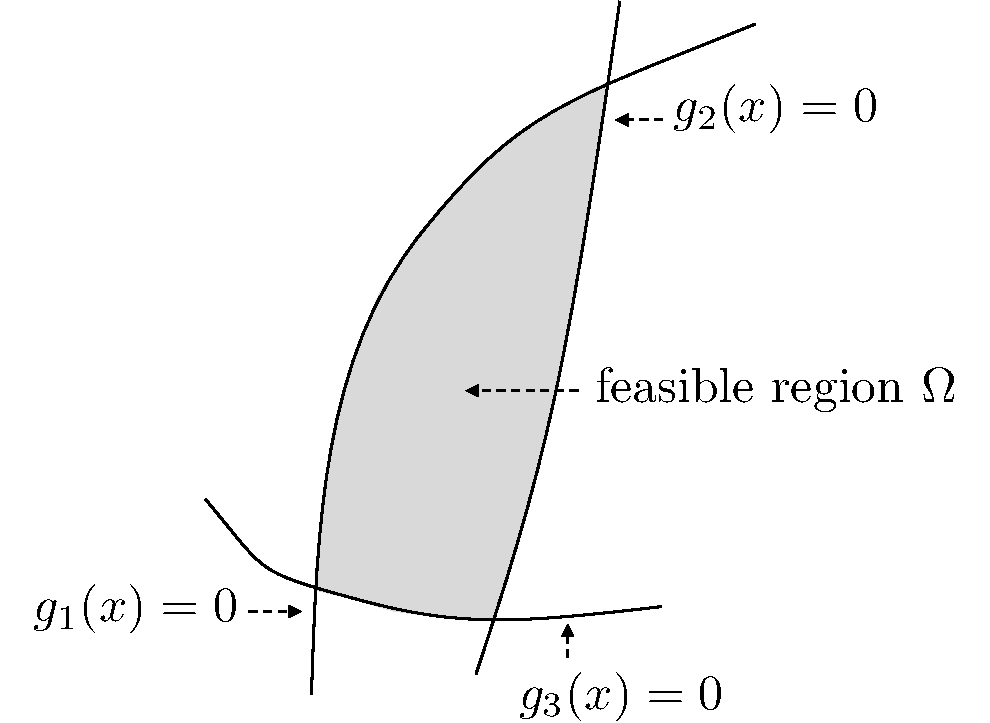
\includegraphics[width=0.99\textwidth]
					{figures/chap18_feasible_region}
			\end{center}			
		\end{column}
	\end{columns}
\end{frame}

%----------------------------------
\begin{frame}\frametitle{Inequality Constraints}
	{\color{blue}Case I.}
	If the local min is in the interior of $\Omega$, then clearly
	\[ 
		\nabla f(x^{\ast}) = 0 
	\]
	or
	\[ 
		\nabla f(x^{\ast}) 
			+ 0 \cdot \nabla g_1(x^{\ast}) 
			+ 0 \cdot \nabla g_2(x^{\ast}) 
			+ 0 \cdot g_3(x^{\ast}) = 0.
	\]
\end{frame}

%----------------------------------
\begin{frame}\frametitle{Inequality Constraints}
	{\color{blue}Case II.}
	The local minimum is on the boundary but not at a corner
	\begin{center}
		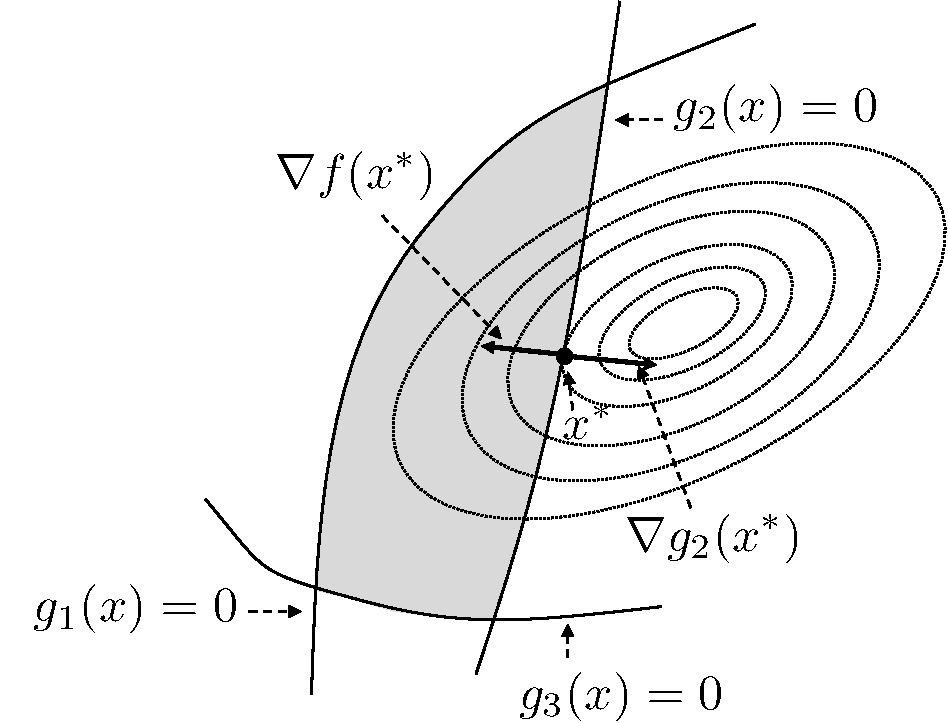
\includegraphics[width=0.5\textwidth]
			{figures/chap18_gradient_of_g}
	\end{center}
	Since in this case $g_1$  is an equality constraint, we must have that $\nabla f(x^{\ast}) \parallel \nabla g_1(x^{\ast})$.  In fact, in this case the two vectors point in opposite directions!  Therefore
	\[
		\nabla f(x^{\ast}) + \mu_1 \nabla g_1(x^{\ast}) + 0\cdot \nabla g_2(x^{\ast}) + 0\cdot g_3 (x^{\ast}) = 0.
	\]	
\end{frame}

%----------------------------------
\begin{frame}\frametitle{Inequality Constraints}
	{\color{blue}Case III.}
		
	\begin{center}
		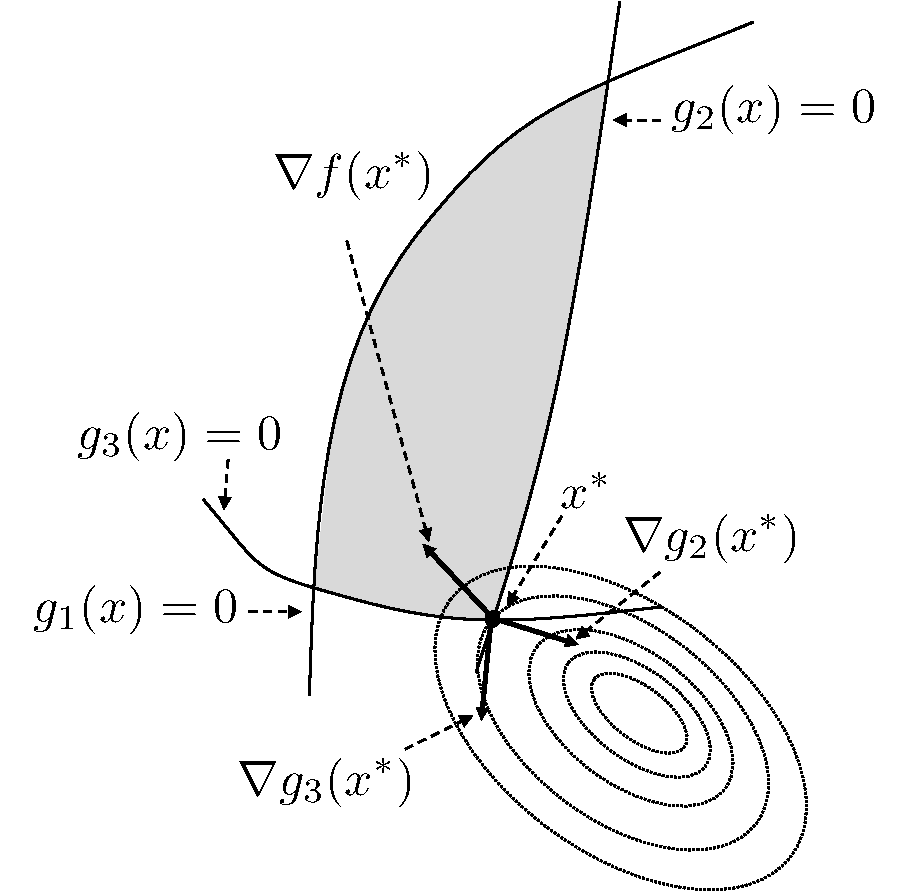
\includegraphics[width=0.5\textwidth]
			{figures/chap18_two_inequality_constraints}
	\end{center}
	In this case, $\nabla f(x^{\ast})$ is in the linear span of $\nabla g_1(x^{\ast})$ and $\nabla g_2(x^{\ast})$ where the coefficients are negative.  Therefore
	\[ 
		\nabla f(x^{\ast}) 
			+ \mu_1 \nabla g_1(x^{\ast}) 
			+ \mu_2 \nabla g_2 (x^{\ast}) 
			+ 0\cdot g_3 (x^{\ast}) = 0 
	\]
	where $\mu_1 > 0$ and $\mu_2 > 0$.
\end{frame}

%----------------------------------
\begin{frame}\frametitle{Inequality Constraints}
	In general, for inequality constraints at a local minimum $x^{\ast}$ we have that
	\begin{enumerate}
	\item $\nabla f(x^{\ast}) + \nabla \gbf(x^{\ast})\mu = 0$
	\item $\gbf(x^{\ast})^\top  \mu = 0$
	\item $\mu \geq 0$
	\end{enumerate}
	
	\vfill

	Conditions (1) and (3) together mean that $\nabla f(x^{\ast})$ is contained in the (negative) linear span of $\{\nabla g_1(x^{\ast}),\ldots,\nabla g_{q}(x^{\ast}) \}$.
	
	\vfill
	
	Condition (2): Note that if the constraint is active, i.e. $g_i(x^{\ast}) = 0$ then $\mu_i$ can be nonzero, but if $g_i$ is inactive, i.e. $g_i(x^{\ast}) < 0$ then $\mu_i$ must be zero to satisfy (2).		
\end{frame}

%----------------------------------
\begin{frame}\frametitle{Inequality Constraints}
	Now lets go back to the general constrained optimization problem:
	\begin{mini*}|s|
		{}{f(x)}{}{}
		\addConstraint{\hbf(x) = 0}
		\addConstraint{\gbf(x) \leq 0}
	\end{mini*}	
	where 
	$f:\mathbb{R}^n\to \mathbb{R}$,
	$h(x):\mathbb{R}^n\to\mathbb{R}^p$,
	$g(x):\mathbb{R}^n\to\mathbb{R}^q$.
	
	\begin{definition}
	$x^{\ast}$ is a \underline{regular point} if $\nabla h_i(x^{\ast}), i = 1, \ldots, p$ and $\nabla g_j(x^{\ast})$ are linearly independent for all $j=1,\dots, q$ such that $g_j(x^{\ast})$ is active.		
	\end{definition}
\end{frame}
	
%----------------------------------
\begin{frame}\frametitle{Inequality Constraints}
	For example, suppose that
	$\hbf = \begin{pmatrix}
	    	h_1\\h_2
	  	 \end{pmatrix}$, and 
	$\gbf = \begin{pmatrix}
	    	g_1\\g_2\\g_3
	  	 \end{pmatrix}$.
	\begin{center}
		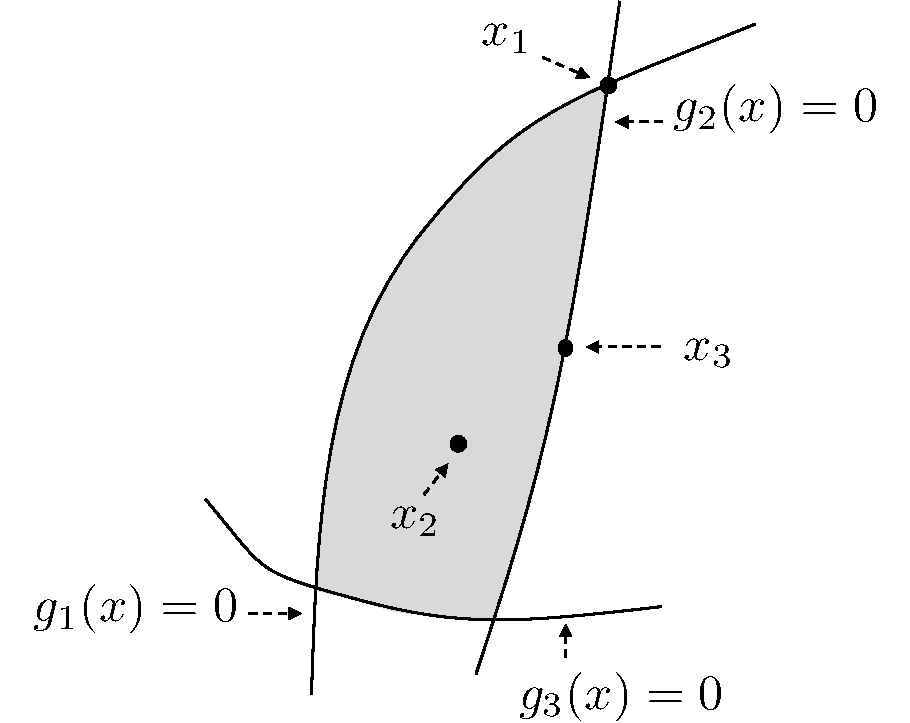
\includegraphics[width=0.4\textwidth]
			{figures/chap18_feasible_points} 
	\end{center}

	  	 
	Then $x^{\ast}$ is a regular point at:
	\begin{itemize}
		\item $x_1$ if 
			$\{ \nabla h_1(x_1), \nabla h_2(x_1), \nabla g_1(x_1), \nabla g_2(x_1) \}$ are  linearly independent.
		\item $x_2$ if 
			$\{ \nabla h_1(x_2), \nabla h_2(x_2) \}$ are linearly independent.
		\item $x_3$ if 
			$\{ \nabla h_1(x_3), \nabla h_2(x_3), \nabla g_1(x_3) \}$ are linearly independent.
	\end{itemize}
\end{frame}

%----------------------------------
\begin{frame}\frametitle{Kuhn Tucker Conditions: Necessary Conditions}	
	\begin{theorem}[Moon Theorem 18.6]
		Let $x^{\ast}$ be a regular local minimum, then 
		$\exists \lambda \in \mathbb{R}^p$ 
		(regular Lagrange multipliers), and
		$\exists \mu \in \mathbb{R}^q$, 
		such that
		\begin{enumerate}
		  \item $\mu \geq 0$ (element wise)
		  \item $\gbf^\top (x^{\ast})\mu = 0$
		  \item $ \nabla f(x^{\ast}) + \nabla \hbf^\top (x^{\ast})\lambda + \nabla \gbf^\top (x^{\ast})\mu = 0$.
		\end{enumerate}		
	\end{theorem}
\end{frame}

%----------------------------------
\begin{frame}\frametitle{Kuhn Tucker Conditions: Sufficient Conditions}	
	\begin{theorem}[Moon 18.7]
		Suppose $f,g,h$ are in $C_2$.
		If there exist $\lambda \in \mathbb{R}^p, \mu \in \mathbb{R}^q$ such that at $x^{\ast}$
		\begin{enumerate}
		  \item $\mu \geq 0$
		  \item $\gbf^\top (x^{\ast})\mu = 0$
		  \item $\nabla f(x^{\ast}) + \nabla \hbf^\top (x^{\ast})\lambda + \nabla \gbf^\top (x^{\ast})\mu = 0$
		  \item $p^\top (\nabla^2f(x^{\ast}) + \sum_{k=1}^p \nabla^2 h_k(x^{\ast})\lambda_k + \sum_{k=1}^q \nabla g_k(x^{\ast})\mu_k )p > 0 $
		\end{enumerate}
		for all $p$ in the tangent plane of the \underline{active} constraints, then $x^{\ast}$ is a local constrained minimum.		
	\end{theorem}
\end{frame}

%----------------------------------
\begin{frame}\frametitle{Kuhn Tucker Conditions: Example 18.9.1}
	\begin{mini*}|s|
		{}{3x_1^2 + 4x_2^2 + 6x_1x_2 - 8x_2 - 6x_1}{}{}
		\addConstraint{x_1^2 + x_2^2 - 9 \leq 0}
		\addConstraint{2x_1 - x_2 - 4 \leq 0}
	\end{mini*}
	The necessary conditions are:
	\begin{align*}
		6x_1 + 6x_2 - 6 + \mu_1(2x_1)+\mu_2(2) &= 0\\
		8x_2 + 6x_1 - 8 + \mu_1(2x_2)+\mu_2(-1) &= 0\\
		\mu_1(x_1^2+x_2^2-9) + \mu_2(2x_1 - x_2 - 4) &= 0 \\
		\mu_1 \geq 0, \mu_2 \geq 0
	\end{align*}
\end{frame}

%----------------------------------
\begin{frame}\frametitle{Kuhn Tucker Conditions: Example 18.9.1}
	Lets try various combinations of active constraints:
	
	\begin{columns}
		\begin{column}{0.5\textwidth}
			\textcolor{blue}{Case I  (Both inactive) 
			i.e. $\mu_1 = \mu_2 \ 0$}
			
			Therefore, must solve
			\begin{align*}
			  6x_1 + 6x_2 - 6 &= 0\\
			  8x_2 + 6x_1 - 8 &= 0\\
			\intertext{i.e.,}\\
			\begin{pmatrix}
			    6 & 6\\
			    6 & 8
			  \end{pmatrix}\begin{pmatrix}
			    x_1\\x_2
			  \end{pmatrix}&=\begin{pmatrix}
			    6\\8
			  \end{pmatrix}\\
			\implies 
			\begin{pmatrix}
			    x_1\\x_2
			  \end{pmatrix}&=\begin{pmatrix}
			    0\\1
			  \end{pmatrix}
			\end{align*}	
		\end{column}
		\begin{column}{0.5\textwidth}
			Check inequality constraints:
			\begin{align*}
				g_1(x) &= 1 - 9 = -8 \leq 0 \\
				g_2(x) &= -1 - 4 \leq 0
			\end{align*}
			Therefore
			\[
				x^{\ast} = \begin{pmatrix}
			    			0\\1
			  			   \end{pmatrix}, 
			  	\mu^{\ast} = \begin{pmatrix}
			    				0\\0
			  			     \end{pmatrix}
			\]
			satisfies necessary conditions.
			
			Sufficient condition:
			\[ 
				\nabla^2 f 
					= \begin{pmatrix}
			    		6 & 6\\
			    		6 & 8
			  		  \end{pmatrix} > 0  
			\]	
			implies local minimum.		
		\end{column}
	\end{columns}
\end{frame}

%----------------------------------
\begin{frame}\frametitle{Kuhn Tucker Conditions: Example }
	\begin{mini*}|s|
		{}{x_1^2 + x_2^2}{}{}
		\addConstraint{x_1 + x_2 + 1 \leq 0}
		\addConstraint{-x_1 + x_2 + 1 \leq 0}
	\end{mini*}

	\begin{center}
		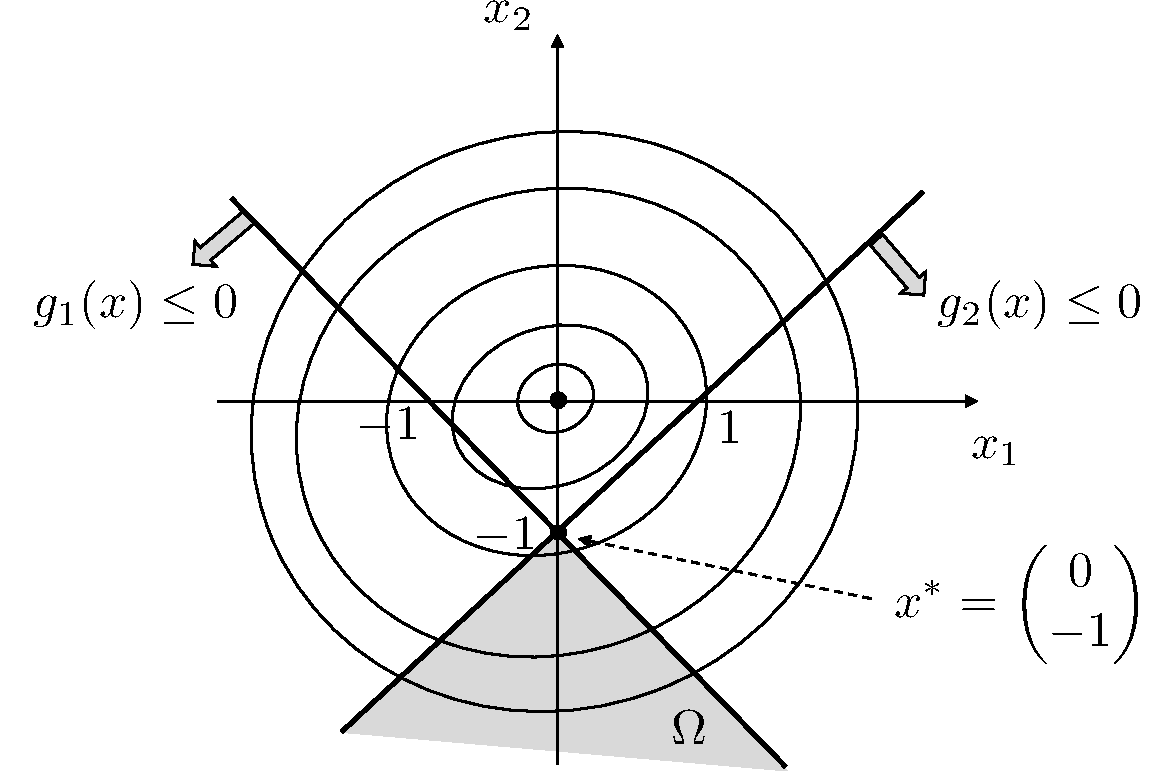
\includegraphics[width=0.5\textwidth]
			{figures/chap18_example2}
	\end{center}
\end{frame}

%----------------------------------
\begin{frame}\frametitle{Kuhn Tucker Conditions: Example }
	The necessary conditions are:
	\begin{align*}
		2x_1 + \mu_1 - \mu_2 &= 0\\
		2x_2 + \mu_1 + \mu_2 &= 0\\
		\mu_1(x_1 + x_2 + 1) + \mu_2(-x_1 + x_2 + 1) &= 0\\
		\mu_1 \geq 0, \mu_2 \geq 0
	\end{align*}	
	Try various combinations of active constraints
	\textcolor{blue}{Case 1: (Both inactive) }
	\begin{align*}
		2x_1 &= 0\\
		2x_2 &= 0
	\end{align*}
	\[ \implies x^{\ast} = \begin{pmatrix}
	    0\\0
	  \end{pmatrix}
	\]
	However, both constraints are violated since
	\begin{align*}
		g_1^{\ast}(x^{\ast}) = 1 \geq 0\\
		g_2(x^{\ast}) = 1 \geq 0.
	\end{align*}
\end{frame}
	
%----------------------------------
\begin{frame}\frametitle{Kuhn Tucker Conditions: Example }
	\textcolor{blue}{Case 2: $g_1$-active, $g_2$-inactive}
	\begin{align*}
		2x_1 + \mu_1 &= 0 \quad\implies x_1 = -\frac{1}{2}\mu_1 \\
		2x_2 + \mu_1 &= 0 \quad\implies x_2 = -\frac{1}{2}\mu_1\\
		\mu_1(x_1 + x_2 + 1) &= 0\\
		\mu_1 > 0
	\end{align*}
	Last two equations imply that
	\[ 
	\mu_1(-\frac{1}{2}\mu_1-\frac{1}{2}\mu_1 + 1) = -\mu_1^2 + \mu_1 = \mu_1(1-\mu_1) = 0.
	\]
	Solving for $\mu_1$ gives $\mu_1 = 0$ or \fbox{$\mu_1 = 1$}.
	Therefore 
	\[
		x^{\ast} = 
			\begin{pmatrix}
	    		-\frac{1}{2} \\
	    		-\frac{1}{2}
	  		\end{pmatrix}
	\]	
\end{frame}

%----------------------------------
\begin{frame}\frametitle{Kuhn Tucker Conditions: Example }
	Checking constraints:
	\begin{align*}
		g_1(x^{\ast}) &= -\frac{1}{2} -\frac{1}{2} + 1 = 0 \leq 0 \qquad \text{ ok }\\
		g_2(x^{\ast}) &= \frac{1}{2} -\frac{1}{2} + 1 = 1 \geq 0 \qquad \text{ no }
	\end{align*}	
	\textcolor{blue}{Case 3: $g_1$-inactive, $g_2$-active}
	 Similar results to Case 2.
	 
	 \vfill

	\textcolor{blue}{Case 4: Both active}
	\begin{align*}
		& \mu_1(\frac{1}{2}\mu_2 - \frac{1}{2}\mu_1 - \frac{1}{2}\mu_2-\frac{1}{2}\mu_1 + 1) \\
		& \quad 
		+ \mu_2(-\frac{1}{2}\mu_2 + \frac{1}{2}\mu_1 - \frac{1}{2}\mu_1 - \frac{1}{2}\mu_2 + 1) = 0 \\
		\implies & \mu_1(1-\mu_1) + \mu_2(1-\mu_2) = 0
	\end{align*}	
\end{frame}
	
%----------------------------------
\begin{frame}\frametitle{Kuhn Tucker Conditions: Example }
	A positive solution is
	\[ 
		\begin{pmatrix}
	    	\mu_1\\
	    	\mu_2
	  	\end{pmatrix} = 
	  	\begin{pmatrix}
	    	1\\1
	  	\end{pmatrix} > 0 
	\]
	which gives
	\[
		x^{\ast} = 
			\begin{pmatrix}
	      		0 \\ -1
	    	\end{pmatrix}
	\]
	
	\vfill
	
	Constraints can be verified to be satisfied.
	
	\vfill
	
	
	Sufficient condition:
	\[ 
		\nabla^2 f + \nabla^2 g \mu = 
			\begin{pmatrix}
	    		2 & 0\\
	    		0 & 2
	  		\end{pmatrix} + 
	  		\begin{pmatrix}
	    		0 & 0\\
	    		0 & 0
	  		\end{pmatrix}1 + 
	  		\begin{pmatrix}
	    		0 & 0\\
	    		0 & 0
	  		\end{pmatrix}1 = 
	  		\begin{pmatrix}
	    		2 & 0\\
	    		0 & 2
	  		\end{pmatrix} > 0
	\]
	Therefore $x^{\ast}$ is a local minimum.	
\end{frame}

\end{document}
